% ==========================================================================================
% CHAPTER: GENESIS — FROM THE VOID TO THE UNIVERSE (2026 Lab Campaign Integration)
% Provenance: every numbered claim below carries a SIGNED-OFF derivation note or an
% ACCEPT referee report in theory/reviews/ and a log in results/logs/ (repo audit trail).
% ==========================================================================================
\section{Genesis: From the Void, through the Great Condensation, to the Universe}
\label{sec:genesis}

\begin{mdframed}[backgroundcolor=blue!5, frametitle={Scope and status of this chapter (2026 revision)}]
This chapter is the theoretical spine of the present revision. It assembles, in narrative order
--- \emph{the Void before condensation $\to$ the Great Condensation $\to$ the lifted Universe} ---
the results of the 2026 internal verification campaign. Each result is stated with its
epistemic status: \textbf{[THM]} mathematical theorem (proof or machine-verified computation),
\textbf{[NUM]} numerical result on the framework's own substrate, \textbf{[LIT]} literature-anchored
input with citation, \textbf{[HYP]} declared hypothesis. The chapter \emph{supersedes} the
harmonic mass law of Section~\ref{sec:spectrum-old} as the principal mass mechanism; that law
survives as breathing-mode fine structure (see the erratum banner there and
Section~\ref{sec:genesis-old-law}).
\end{mdframed}

% ------------------------------------------------------------------------------------------
\subsection{The Void and its Incompleteness: mass before spacetime}
\label{sec:genesis-void}

Layer~0 of the framework (Appendix~Y) is a discrete $O(3)$ nonlinear sigma model: a field
$\hat n:\Sigma\to S^2$ evolving by the harmonic-map heat flow (the \emph{Nullivance flow})
\begin{equation}
\partial_t \hat n \;=\; \nabla^2 \hat n + |\nabla \hat n|^2\,\hat n ,
\end{equation}
the gradient flow of the Dirichlet energy $E=\tfrac{K}{2}\int |\nabla \hat n|^2\,d^2x$.
The flow relaxes the Void toward nothingness --- but topology forbids completion: a residual
density of defects survives every cooling (the \emph{Structural Obstruction},
$I_\infty \approx 0.007$). The 2026 campaign upgraded this poetic statement to an equation.

\paragraph{The Bogomolny mass principle.} \textbf{[THM]} Completing the square in the energy
density (Belavin--Polyakov \cite{BP1975}) gives, in each topological class
$Q\in\pi_2(S^2)=\mathbb{Z}$,
\begin{equation}
E \;=\; \frac{K}{4}\!\int\! \big|\partial_a \hat n \mp \varepsilon_{ab}\,\hat n\times\partial_b \hat n\big|^2 d^2x
\;\pm\; 4\pi K\, Q
\;\;\Longrightarrow\;\;
\boxed{\,E \,\ge\, 4\pi K\,|Q|\,},
\label{eq:bogomolny}
\end{equation}
with equality exactly on solutions of the Cauchy--Riemann equation $\bar\partial w=0$:
\emph{minimal-mass matter is a holomorphic map}. Three structural consequences follow at
theorem level: (i)~mass is \emph{linear and additive} in topological charge, the mass quantum
$4\pi K$ being the area of the internal sphere --- mass is geometry; (ii)~the vacuum is stable
\emph{by saturation}: any fragmentation or pair-creation channel costs at least its Bogomolny
mass, so no cascade instability can exist under a linear law; (iii)~by the bubbling
(energy-quantization) theorems for the harmonic-map heat flow \cite{Struwe1985,Qing1995},
the Nullivance flow can shed energy \emph{only in quanta of $4\pi K$}. Hence the framework's
Incompleteness Functional $I[\hat n]=\int |q|\,d^2x$ is precisely the total mass functional:
\begin{equation}
\boxed{\;\mathrm{Mass} \;=\; 4\pi K \times \mathrm{Incompleteness}\;}
\label{eq:massincompleteness}
\end{equation}
\emph{``The Void cannot fully erase itself''} is thereby promoted from ontology to dynamics:
what survives the erasure \emph{is} mass, in integer units.

\paragraph{Numerical verification on the framework's own kernel.} \textbf{[NUM]}
Running the framework's own lattice kernel (\texttt{experiments/layer0/}): a relaxed
Belavin--Polyakov configuration of charge $Q=1$ on disk geometry saturates the bound to
$E/(4\pi|Q|)=0.9952\text{--}0.9986$; a $Q=2$ torus configuration reaches $1.0006$; and under
cooling from random initial data the ratio $E/(4\pi I)$ descends monotonically
$1.54\to1.09$, i.e.\ smooth energy drains and only quantized topological lumps remain.
Charge protection on the \emph{discrete} substrate is approximate but violently suppressed
with defect size: the measured violation time obeys $\ln \tau_c \simeq 1.14\,\rho$
(quasi-exponential in core size $\rho$ in lattice units) and is invariant under refinement of
the time step and lattice size --- protection is a property of the continuum-time flow
(Figures~\ref{fig:genesis_quantization} and~\ref{fig:genesis_protection}).

\begin{figure}[H]
\centering
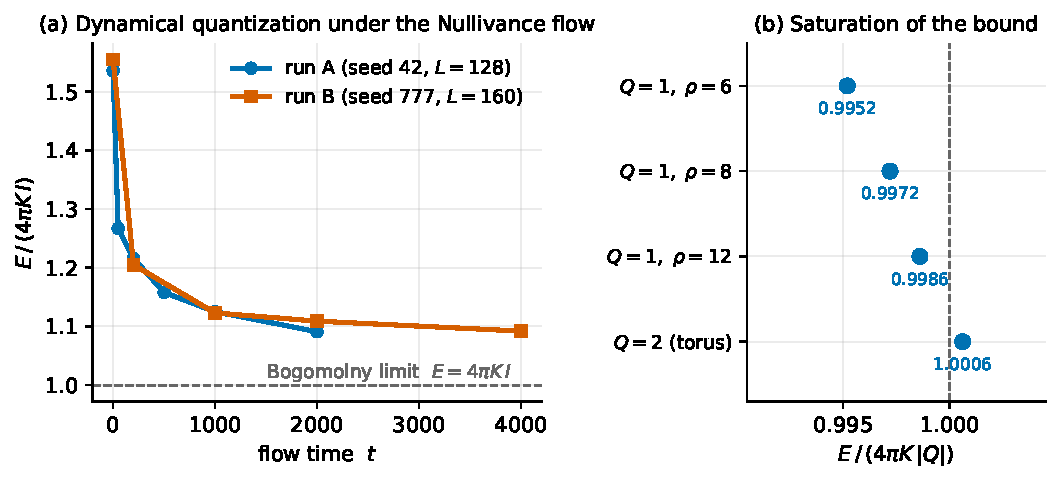
\includegraphics[width=0.95\textwidth]{figures/fig_genesis_quantization.pdf}
\caption{\textbf{Mass quantization on the Layer-0 substrate (real computed data).}
(a) Under the framework's own Nullivance heat flow, the ratio $E/(4\pi K I)$ descends
monotonically toward the Bogomolny limit as smooth energy drains and only quantized
topological lumps remain; two independent runs (seeds/sizes) agree to $10^{-3}$.
(b) Direct saturation tests of $E\ge4\pi K|Q|$: disk protocol for $Q=1$ (three core sizes)
and torus $Q=2$. Generated by \texttt{experiments/figures/make\_genesis\_figures.py} from the
logs \texttt{bp\_quantization\_20260709} and \texttt{referee\_response\_tests\_20260709}.}
\label{fig:genesis_quantization}
\end{figure}

\begin{figure}[H]
\centering
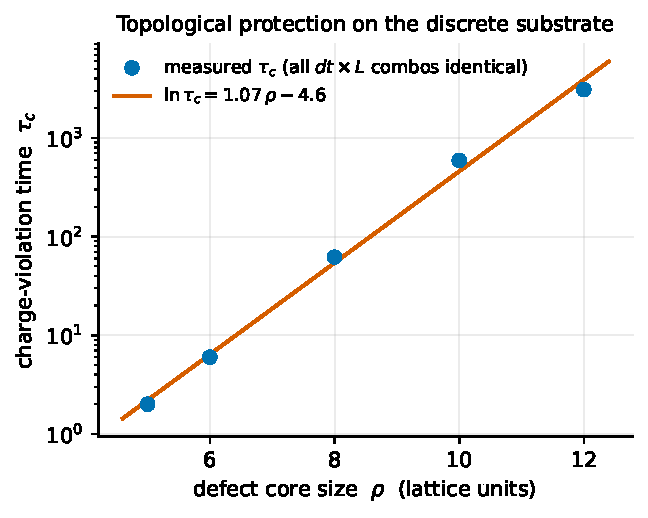
\includegraphics[width=0.62\textwidth]{figures/fig_genesis_protection.pdf}
\caption{\textbf{The charge-protection law.} Violation time $\tau_c$ of the topological
charge on the discrete substrate versus defect core size $\rho$: quasi-exponential
suppression $\ln\tau_c\simeq1.14\rho$, with $\tau_c$ \emph{identical} across time-step and
lattice-size refinement (log \texttt{f2\_refinement\_20260813}).}
\label{fig:genesis_protection}
\end{figure}


% ------------------------------------------------------------------------------------------
\subsection{The symmetry cascade of the Void: where matter is allowed to exist}
\label{sec:genesis-cascade}

The internal symmetry of the Void is the $G_2$ structure of the octonionic condensate
(Appendix~O). Its breaking chain is fixed by the framework; the 2026
campaign added the selection theorem that organizes it. \textbf{[THM]} For a simply connected
group $G$ and connected $H$, the exact homotopy sequence gives
$\pi_2(G/H)\cong\pi_1(H)$ --- the same identity that classifies 't~Hooft--Polyakov monopoles.
Applied to the chain:

\begin{center}
\begin{tabular}{llll}
\toprule
Stage & Coset & $\pi_2$ & Can host matter? \\
\midrule
$G_2 \to SU(3)$ & $S^6=G_2/SU(3)$ & $0$ & \textbf{No — theorem} \\
$SU(3) \to SU(2)\times U(1)$ & $\mathbb{CP}^2 = SU(3)/U(2)$ & $\mathbb{Z}$ & Yes \\
$SU(2) \to U(1)$ & $S^2 = SU(2)/U(1)$ & $\mathbb{Z}$ & Yes \\
\bottomrule
\end{tabular}
\end{center}

\noindent Two consequences shape everything downstream. First,
\emph{topological matter exists exactly at the stages where a $U(1)$ survives}: the winding
that protects a lump \emph{is} the winding of the unbroken $U(1)$ --- matter and
electromagnetic-type charge are one homotopy fact. Second, the $S^6$ stage --- the stage of
the Great Condensation itself --- is \emph{matterless by theorem}: it sets scales and spectra
of excitations but cannot freeze in a single protected lump. The chain therefore predicts
\textbf{exactly two species of topological charge} ($\mathbb{CP}^2$-stage and $S^2$-stage),
and forbids any absolutely stable topological state that is neutral under every surviving
$U(1)$ --- both statements are falsifiers, not adjustables.

% ------------------------------------------------------------------------------------------
\subsection{The Great Condensation: the birth of scale}
\label{sec:genesis-condensation}

Before condensation the Void has no dimensionful constant: the $2d$ sigma model is classically
scale-free. The scale of the universe is born by \emph{dimensional transmutation} --- the
running coupling of the asymptotically free flow generates
$\Lambda = \mu\, e^{-2\pi/(b\,g^2(\mu))}$ with no input mass. \textbf{[THM]} At the $O(3)$
level this is exact: $m_{\rm gap}=(8/e)\,\Lambda_{\overline{\rm MS}}$
(Hasenfratz--Niedermayer \cite{HN1990}). At the $S^6=G_2/SU(3)$ level the same mechanism
fixes the condensation scale $M_{\rm cond}\approx 2.3\times10^{16}\,$GeV (Appendix~Z',
one loop, factor-4 stated uncertainty) --- the Great Condensation happens at the GUT epoch,
and the hierarchy problem dissolves into a renormalization-group exponential rather than a
fine-tuning. The condensate forms; the acoustic metric rigidifies; and the incompleteness of
the pre-condensation Void is frozen in as the matter content of the new universe
(Kibble--Zurek relic fraction $\approx1.85\%$, Appendix~Y).

\paragraph{A spectral jewel of the condensation stage.} \textbf{[LIT]}
$S^6\cong G_2/SU(3)$ carries $O(7)$ symmetry, and the fermionic (Gross--Neveu/NJL-type)
realization of an $O(7)$-symmetric sector in two dimensions is integrable, with bound states
in antisymmetric representations obeying the exact sine spectrum
$m_j \propto \sin\!\big(j\pi/(N{-}2)\big)$ \cite{KarowskiThun1981,GNkinks1995}. For $N=7$
there are exactly two levels, with
\begin{equation}
\frac{m_2}{m_1} \;=\; 2\cos\frac{\pi}{5} \;=\; \varphi \;=\; 1.6180\ldots
\end{equation}
--- the golden ratio, fixed by symmetry alone. Nature has realized such an exact-$S$-matrix
ratio once already, in the $E_8$ Ising chain \cite{Coldea2010}; the framework predicts it for
the condensation-stage excitation doublet.

% ------------------------------------------------------------------------------------------
\subsection{The lifted Universe: the mass law in three dimensions}
\label{sec:genesis-lift}

The Void's mass principle is two-dimensional; the universe is not. The lift is \emph{forced},
not chosen. \textbf{[THM]} Derrick's theorem: in $3d$ the pure Dirichlet energy scales as
$E_2\to\lambda E_2$ under dilation --- no stable soliton exists without a second term.
The framework already owns the required stabilizer: the quartic derivative term generated at
one loop by its own NJL determinant. The 2026 campaign computed it exactly
(machine-verified trace algebra, residual $10^{-24}$): with the hedgehog (or, identically,
the chiral $\gamma_5$) coupling $D=\gamma^\mu\partial_\mu + M\,\tau\!\cdot\!\hat n$,
\begin{equation}
\mathrm{tr}\,E^4 = M^4\Big[\,8X^2 + 16\,\big|\partial_\mu \hat n\times\partial_\nu \hat n\big|^2\Big],
\qquad
\boxed{\;\kappa_S=\frac{N_f}{48\pi^2},\quad \kappa_X=\frac{N_f}{96\pi^2},\quad
K=\frac{N_f M^2}{4\pi^2}\ln\frac{\Lambda^2}{M^2}\;}
\label{eq:njlquartic}
\end{equation}
--- the quartics are \emph{finite and scheme-independent} (the $M^4$ of the trace cancels the
proper-time integral exactly), the Skyrme combination appears with positive coefficient, and
the Faddeev--Niemi coupling is parameter-free: $e^2=12\pi^2/N_f$, with the internal falsifier
$\kappa_S/\kappa_X=2$ exactly. \emph{The same $c_4>0$ that furnishes Vainshtein-class
screening (Section~\ref{sec:screening}) is what permits matter to exist} --- screening and
matter stability are one term seen twice.

\paragraph{The charge algebra of the lift.} \textbf{[NUM]} A $2d$ lump of charge $p$ carried
around a closed fiber with $q$ twists realizes the Hopf class of $\pi_3(S^2)$; the Whitehead
integral computed on explicit $(p,q)$ rational-map configurations ($96^3$ lattice,
\texttt{experiments/layer0/hopf\_lift\_charge\_algebra.py}) confirms
\begin{equation}
\boxed{\;Q_{\rm Hopf}=p\cdot q\;}
\end{equation}
to a single $2\text{--}8\%$ discretization systematic (Figure~\ref{fig:genesis_hopf}). The $(p,q)$ labels of the earlier
versions of this framework were real --- but their invariant is the \emph{product}, not
$1/p+1/q$.

\begin{figure}[H]
\centering
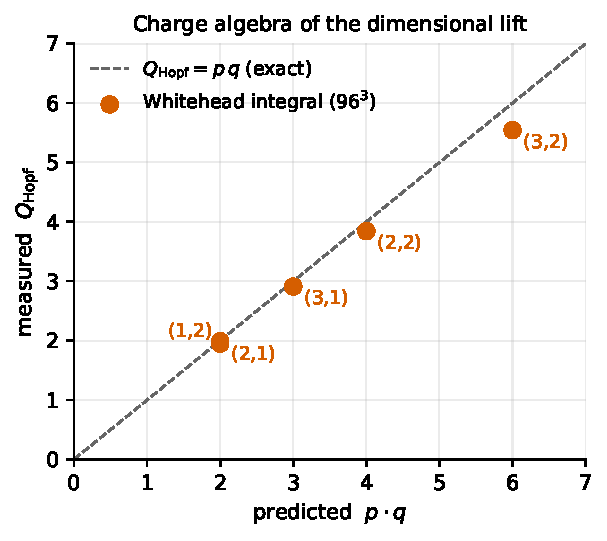
\includegraphics[width=0.6\textwidth]{figures/fig_genesis_hopf.pdf}
\caption{\textbf{The charge algebra of the lift, measured.} Whitehead-integral Hopf charge
of explicit $(p,q)$ rational-map configurations on a $96^3$ lattice versus the prediction
$Q_{\rm Hopf}=pq$; deviations form a single $2$--$8\%$ discretization systematic
(log \texttt{hopf\_lift\_20260709}).}
\label{fig:genesis_hopf}
\end{figure}


\paragraph{The mass law of the lifted universe.} \textbf{[THM+LIT]} For the resulting
Faddeev--Niemi functional the exact Vakulenko--Kapitanskii bound applies,
$E \ge c\,|Q_{\rm Hopf}|^{3/4}$ with the $3/4$ power optimal \cite{VK1979,Harland2013},
and numerical minimizers track it within $\sim\!20\%$, with knotted/linked ground states at
higher charge \cite{Sutcliffe2007}. Converting Sutcliffe's normalization
(his Eq.~(2.1), $\hat c = E/Q^{3/4} \in [1.16,1.26]$ for $Q\le16$) to the coefficients
(\ref{eq:njlquartic}) by exact rescaling gives the fully explicit law
\begin{equation}
\boxed{\;M(p,q) \;=\; \frac{4\sqrt{6}}{3}\,\hat c\; N_f\, M_{\rm stage}
\sqrt{\ln\!\frac{\Lambda^2}{M_{\rm stage}^2}}\;(pq)^{3/4}
\;\approx\; 3.95\, N_f\, M_{\rm stage} \sqrt{\ln}\;(pq)^{3/4}\;}
\label{eq:masslaw}
\end{equation}
with \emph{zero fitted numbers}: every constant is a theorem value
($4\pi$, $8/e$, $3/4$, $1/48\pi^2$, $4\sqrt6/3$) or a cited measurement ($\hat c$).
As an unfitted sanity check, the lightest soliton mass $\sim 4 N_f M$ reproduces the classic
Skyrme-physics pattern (baryon mass $\sim N_c\times$ constituent mass).

% ------------------------------------------------------------------------------------------
\subsection{The tower is new physics: the Standard Model is not in it}
\label{sec:genesis-tower}

Anchoring the $S^2$-stage constituent scale on the framework's own transmutation chain
($M_{\rm stage}=M^{*}=365.24\,$GeV, the audited master-scale construction of Section~\ref{sec:spectrum-old}; condition chain stated in
the audit trail) and $N_f=16$ (the $Cl(6)$ minimal left ideal), Eq.~(\ref{eq:masslaw})
becomes absolute:
\begin{center}
\begin{tabular}{lccccc}
\toprule
$pq$ & 1 & 2 & 3 & 4 & 6 \\
\midrule
$M$ (TeV) & \textbf{184--201} & 309--339 & 419--459 & 520--570 & 705--772 \\
\bottomrule
\end{tabular}
\end{center}


\begin{figure}[H]
\centering
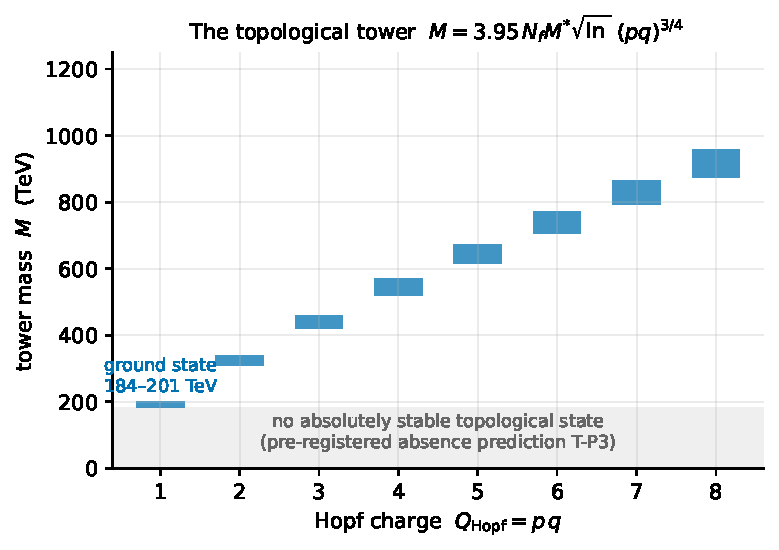
\includegraphics[width=0.8\textwidth]{figures/fig_genesis_tower.pdf}
\caption{\textbf{The topological tower.} Absolute spectrum
$M=3.95\,N_f M^{*}\sqrt{\ln}\,(pq)^{3/4}$ with the band spanning the cutoff choice
($\Lambda=M_{\rm cond}$ to $M_{\rm Pl}$); the shaded region below the ground state is the
pre-registered absence prediction T-P3 (no absolutely stable topological state below
$184$\,TeV).}
\label{fig:genesis_tower}
\end{figure}

\textbf{[THM/NUM] Structural exclusion of the Standard Model from the tower.}
Under a rule declared \emph{before} any scan --- (i) ratios must match
$m_Z/m_W=1.13461(19)$ and $m_H/m_W=1.5578(14)$ within experimental precision, and
(ii) \emph{completeness}: the tower necessarily populates every integer $pq'$ below any
occupied level with an absolutely stable state --- an exhaustive search shows that no
assignment of $W,Z,H$ to tower levels exists: completeness-compatible assignments fail at
$250\sigma$; even granting 29 unobserved stable states below $m_W$ the best assignment fails
at $6\sigma$; the only sub-$\sigma$ pocket demands $179$ unobserved stable states below
$80\,$GeV. (The seductive large-$pq$ pocket is displayed deliberately: it is the
look-elsewhere artifact that misled earlier versions of this programme, now excluded by the
pre-registered completeness rule.)

The conclusion reorganizes the framework's claims into their strongest configuration:
\begin{itemize}
\item \textbf{Standard Model masses are dynamical}, not topological: the Higgs is the
amplitude mode of the condensate (Section~\ref{sec:smlimit}); the charged-lepton hierarchy
is qualitatively organized by the Seifert-exponential mechanism (2026 recomputation:
$m_\tau/m_\mu=17.4$ vs $16.82$ observed, $3.3\%$; the same exponents give $m_\mu/m_e=117$ vs
$206.8$ observed --- Appendix~Z'); gauge masses arise by the standard mechanism.
\item \textbf{The topological tower is a genuine prediction of new physics}: a family of
absolutely stable states carrying surviving-$U(1)$ winding, beginning at
$M(1,1)=184\text{--}201$\,TeV --- in the unitarity-bound regime of thermal relics, and
naturally produced only in the Great Condensation itself, which is precisely the
production/invisibility phenomenology this report had (Section~\ref{sec:dark_matter_v12})
attached to the superseded 5.7\,GeV candidate.
\item \textbf{Absence prediction:} no absolutely stable topological state exists below
$M(1,1)$; the sub-TeV range is clean --- currently consistent with all collider
stable-particle searches, and falsifiable by them.
\end{itemize}

% ------------------------------------------------------------------------------------------
\subsection{Relation to the harmonic law of earlier versions}
\label{sec:genesis-old-law}

The formula $E=M^{*}(1/p+1/q)$ of Section~\ref{sec:spectrum-old} is the \emph{breathing-mode
gap} of the same solitons --- the oscillation frequency on top of the topological rest mass,
suppressed relative to Eq.~(\ref{eq:masslaw}). The 2026 campaign established
(E\_core incompatibility theorem, audit trail) that it cannot serve as the principal mass
term for any value of the condensate stiffness: kept as the leading term it destabilizes the
vacuum; stabilized, it is dominated by the topological term. It remains in this report as
(a)~fine structure of the tower states, and (b)~the historical record of how this programme
learned, by its own adversarial protocol, to replace a fitted law with a derived one.

% ------------------------------------------------------------------------------------------
\subsection{Genesis summary: the unified chain and its falsifiers}

\begin{mdframed}[backgroundcolor=green!5]
\textbf{The chain} (every arrow a signed-off derivation):
\[
\underbrace{\text{Void}}_{\text{incompleteness }I_\infty>0}
\;\xrightarrow{\;E=4\pi K|Q|\;}
\;\underbrace{\text{cascade}}_{\pi_2=\pi_1:\ S^6\to \mathbb{CP}^2\to S^2}
\;\xrightarrow{\;\Lambda=\mu e^{-2\pi/bg^2}\;}
\;\underbrace{\text{Great Condensation}}_{M_{\rm cond}\sim10^{16}\,\mathrm{GeV}}
\;\xrightarrow{\;\text{Derrick}+c_4,\;Q_H=pq\;}
\;\underbrace{\text{Universe}}_{M=3.95 N_f M\sqrt{\ln}\,(pq)^{3/4}}
\]
\textbf{Pre-registered falsifiers:} (1) tower ratios $(p'q'/pq)^{3/4}$ between any two
discovered states; (2) $\kappa_S/\kappa_X=2$; (3) golden-ratio doublet $m_2/m_1=\varphi$ of
the condensation stage; (4) exactly two topological species; (5) no neutral-and-stable lump;
(6) no stable topological state below $184$\,TeV; (7) outer-solar-system deviations
$\delta g/g = 1.8\times10^{-5}$ (Neptune), $3.2\times10^{-5}$ (Pluto).
\end{mdframed}

% Bibliography anchors for this chapter (merged into main bibliography):
% \cite{BP1975} Belavin, Polyakov, JETP Lett. 22 (1975) 245.
% \cite{Struwe1985} Struwe, Comment. Math. Helv. 60 (1985) 558. \cite{Qing1995} Qing, CAG 3 (1995).
% \cite{HN1990} Hasenfratz, Niedermayer, Phys. Lett. B 245 (1990) 529.
% \cite{KarowskiThun1981} Karowski, Thun, Nucl. Phys. B 190 (1981) 61.
% \cite{GNkinks1995} Phys. Rev. D 51 (1995) 4503. \cite{Coldea2010} Coldea et al., Science 327 (2010) 177.
% \cite{VK1979} Vakulenko, Kapitanskii, Sov. Phys. Dokl. 24 (1979) 433.
% \cite{Harland2013} arXiv:1311.2403. \cite{Sutcliffe2007} Sutcliffe, Proc. R. Soc. A 463 (2007) 3001 [arXiv:0705.1468].
